\documentclass[11pt,a4paper]{article}

\usepackage[T1]{fontenc}
\usepackage[utf8]{inputenc}
\usepackage{lmodern}
\usepackage{microtype}
\usepackage[margin=2.4cm]{geometry}
\usepackage{amsmath,amssymb,amsfonts}
\usepackage{bm}
\usepackage{booktabs}
\usepackage{multirow}
\usepackage{graphicx}
\usepackage{xcolor}
\usepackage[font=small,labelfont=bf]{caption}
\usepackage{subcaption}
\usepackage{algorithm}
\usepackage{algpseudocode}
\usepackage[numbers,sort&compress]{natbib}
\usepackage[colorlinks=true,linkcolor=blue!50!black,citecolor=blue!50!black,urlcolor=blue!50!black]{hyperref}
\usepackage{cleveref}
\usepackage[section]{placeins}

\graphicspath{{figures/}}

\newcommand{\pcm}{\ensuremath{\,\mathrm{pcm}}}
\newcommand{\dd}{\mathrm{d}}
\newcommand{\Norman}{\textsc{Norman}}

\title{\Norman: A Verified Reduced-Order Benchmark\\
for Pressurized Water Reactor Load-Following Control\\
with Axial Xenon Dynamics}
\author{Isa Maharramov\\[2pt]
\small\url{https://github.com/IsaMaharramov/Norman-The-Machine}}
\date{}

\begin{document}
\maketitle

\begin{abstract}
Grids with a growing share of variable renewable generation need nuclear plants that
follow load: they must change power by tens of percent within hours while respecting
thermal, rate and power-distribution limits, and while xenon-135 builds up and
redistributes in the core. Learned controllers are increasingly proposed for this task,
yet they are evaluated on bespoke, unpublished plant models that cannot be compared or
checked. We present \Norman, an open benchmark for pressurized water reactor (PWR)
load following built on a transparent, verified reduced-order model. Its plant combines
six-group point kinetics, two-node thermal feedback, the I-135/Xe-135 and Pm-149/Sm-149
chains, an S-curve control bank and soluble boron, integrated by an L-stable
second-order SDIRK scheme. An optional one-dimensional axial core, coupled
quasi-statically through a one-group diffusion eigenvalue problem, reproduces axial
xenon oscillations with periods of 24.7--26.0\,h and an S-shaped
integral rod worth that emerges from the flux shape rather than being prescribed. An
optional secondary side, with steam generators, a pressure-limited turbine and steam
properties from IAPWS-IF97, makes the reactor follow the turbine through moderator
feedback, as a real PWR does.
Every numerical component is verified against analytic results: the inhour equation
(error below 0.10\%), the closed-form xenon transient after shutdown (below
0.01\%), and the second-order convergence of the eigenvalue (observed
order 1.999). The task is posed as a constrained Markov decision process with
separate reward and safety cost, four grid scenarios and three fuel-cycle states. We
report baselines for a classical rod/boron controller, Soft Actor-Critic, and a
Simplex-style runtime-assurance shield. The shield removes every reactor trip of the
learned controller (5 of 36 benchmark days without it,
0 with it) but does not make it competitive with the classical
baseline. On the axial task, the classical controller tracks power to within
0.61\% RMS yet violates the axial-offset band in 39\% of all
minutes, leaving a clear and physically meaningful gap for advanced controllers. On
the plant task, controlling reactor power lets the average coolant temperature drift
50\,K off its program, while a temperature controller holds it within 1\,K.
\end{abstract}

\section{Introduction}

Nuclear plants were long operated at constant full power. In France and Germany,
however, PWRs have followed load for decades, and the economic case for flexible
operation is growing with the share of solar and wind generation~\cite{nea2011}. The
European Utility Requirements specify the manoeuvrability expected of a modern plant:
a daily cycle between 100\% and 50\% power and ramps of up to 5\% of rated power per
minute~\cite{eur}. Meeting these requirements is a control problem with three
difficult features:
\begin{enumerate}
  \item \textbf{Slow, hidden dynamics.} Xenon-135, produced mostly through the decay
  of iodine-135, responds to a power change over many hours. Its negative reactivity
  after a power reduction can exceed the available control margin.
  \item \textbf{Actuator limits.} Control rods act quickly but have finite travel and
  distort the power shape. Soluble boron is uniform but slow, and at end of cycle
  there is almost none left to dilute.
  \item \textbf{Spatial instability.} Large PWRs are tall compared with the neutron
  migration length, so xenon can drive slowly growing \emph{axial} oscillations of
  the power distribution~\cite{randall1958,stacey2018}. Operators must keep the axial
  offset in a narrow band.
\end{enumerate}

Learned controllers, reinforcement learning in particular, are attractive for problems
with long horizons and non-linear, partially observed dynamics. Progress in other
fields has relied on shared benchmarks with standard interfaces~\cite{towers2024} and
explicit safety constraints~\cite{garcia2015}. For reactor control, no such benchmark
exists: published studies use plant models that are not released, not verified, or
both. This makes results impossible to compare, and the credibility of the plant
model, which reactor engineers will judge first, is rarely established.

\paragraph{Contributions.} This paper presents \Norman, an open benchmark with four
properties:
\begin{itemize}
  \item A documented reduced-order PWR model (\cref{sec:model}) with an optional
  quasi-static axial core (\cref{sec:axial}) and an optional secondary side
  (\cref{sec:secondary}). Every parameter has a stated source.
  \item A verification suite (\cref{sec:verification}) that compares each numerical
  component against analytic results and against an independent implementation that
  shares no numerical method with the production solver.
  \item A constrained Markov decision process (CMDP) formulation (\cref{sec:task})
  with grid scenarios, fuel-cycle variation, a reactor trip, and safety costs reported
  separately from reward.
  \item Reference controllers and results (\cref{sec:baselines,sec:results}): a
  classical rod/boron controller, Soft Actor-Critic, and a runtime-assurance shield,
  evaluated with a reproducible protocol.
\end{itemize}
The model is intended for control research. It is verified, meaning its equations are
solved correctly; it is not validated against plant data, and it must not be used for
safety analysis (\cref{sec:limitations}).

\section{Plant model}\label{sec:model}

The plant is a generic 3\,GWth four-loop PWR. Parameters are representative
open-literature values (\cref{tab:params}) and do not describe any specific plant.

\subsection{Neutron kinetics}

With normalized fission power $n$ (1 = rated) and six delayed-neutron precursor groups,
\begin{equation}
  \frac{\dd n}{\dd t} = \frac{\rho - \beta}{\Lambda}\, n + \sum_{i=1}^{6} \frac{\beta_i}{\Lambda}\, c_i + S,
  \qquad
  \frac{\dd c_i}{\dd t} = \lambda_i\,(n - c_i),
  \label{eq:pk}
\end{equation}
where the precursors are scaled, $c_i \equiv \Lambda\lambda_i C_i/\beta_i$, so that
$c_i = n$ at equilibrium and every state is of order one. The group data are Keepin's
U-235 thermal values~\cite{keepin1965}. The small intrinsic source $S$ keeps a deeply
subcritical core at a positive, physical power level. It shifts the critical state by
only $-\Lambda S/n \approx 10^{-11}$, which is accounted for exactly when the plant is
initialized.

\subsection{Thermal feedback}

Fuel and coolant are lumped into one node each:
\begin{align}
  C_f \frac{\dd T_f}{\dd t} &= f_f P_0 n - hA\,(T_f - T_c), \\
  C_c \frac{\dd T_c}{\dd t} &= (1 - f_f) P_0 n + hA\,(T_f - T_c) - 2\dot m c_p\,(T_c - T_{in}),
\end{align}
where $T_c$ is the average coolant temperature, so that the core temperature rise is
$2(T_c - T_{in})$. The conductance $hA$ and the flow capacity $\dot m c_p$ follow from
the nominal temperatures, so the full-power steady state is exact by construction.

\subsection{Fission-product poisons}

With local flux $\varphi = n\varphi_0$, dividing the iodine, xenon, promethium and
samarium balances by their full-power equilibrium values gives
\begin{align}
  \frac{\dd I}{\dd t} &= \lambda_I (n - I), &
  \frac{\dd X}{\dd t} &= \kappa\left(\tfrac{\gamma_X}{\gamma} n + \tfrac{\gamma_I}{\gamma} I\right) - (\lambda_X + \sigma_X\varphi_0 n)\, X, \label{eq:xenon}\\
  \frac{\dd P_m}{\dd t} &= \lambda_{Pm} (n - P_m), &
  \frac{\dd S_m}{\dd t} &= \sigma_{Sm}\varphi_0\,(P_m - n S_m),
\end{align}
with $\gamma = \gamma_I + \gamma_X$ and $\kappa = \lambda_X + \sigma_X\varphi_0$. The
macroscopic fission cross-section cancels. The equilibrium xenon and samarium worths
follow from the yields~\cite{lamarsh2001},
\begin{equation}
  w_X = \frac{\gamma}{\nu}\,\frac{\sigma_X\varphi_0}{\lambda_X + \sigma_X\varphi_0} = 2356\pcm,
  \qquad
  w_{Sm} = \frac{\gamma_{Pm}}{\nu} \approx 465\pcm.
\end{equation}

\subsection{Reactivity and actuators}

The total reactivity is
\begin{equation}
  \rho = \rho_{b} + \rho_{rod}(z) + \alpha_B B + \alpha_f (T_f - T_{f,0}) + \alpha_m (T_c - T_{c,0}) - w_X X - w_{Sm} S_m,
  \label{eq:rho}
\end{equation}
where the control-bank insertion $z\in[0,1]$ has the standard S-shaped integral worth
$\rho_{rod}(z) = -W\left(z - \sin(2\pi z)/2\pi\right)$. The bias $\rho_b$ stands for the
excess reactivity of the fuel and is solved at every reset so that the initial state
is exactly critical. Rods move at most $1/180$ of the stroke per second. Boron
changes by at most $3$\,ppm/min and cannot fall below zero. That floor is why load
following becomes difficult at the end of the cycle.

Three fuel-cycle states (beginning, middle and end of cycle; BOC, MOC, EOC) change
$\beta$, $\Lambda$, the feedback coefficients and the initial boron
(\cref{tab:params}). A randomized mode draws a state and perturbs the coefficients by
$\pm 10\%$ to test robustness.

\begin{table}[!htbp]
  \centering
  \caption{Plant parameters. Triplets give BOC / MOC / EOC values.}
  \label{tab:params}
  \small
  \begin{tabular}{@{}llp{6.2cm}@{}}
    \toprule
    Parameter & Value & Source / rationale \\
    \midrule
    $\beta_i/\beta$, $\lambda_i$ & Keepin 6-group & U-235 thermal fission~\cite{keepin1965} \\
    $\beta$ & 0.0065 / 0.0058 / 0.0052 & Falls as Pu-239 builds up \\
    $\Lambda$ & 22 / 20 / 17\,\textmu s & Typical LWR \\
    $P_0$ & 3000\,MWth & Four-loop PWR \\
    $T_{in}$, $T_{c,0}$, $T_{f,0}$ & 292, 308, 650\,$^\circ$C & Cold leg, core average, fuel average \\
    $C_f$, $C_c$ & $4.27\times10^{7}$, $1.2\times10^{8}$\,J/K & Fuel time constant $\approx 5$\,s \\
    $\alpha_f$ & $-2.2$ / $-2.5$ / $-2.9$\,pcm/K & Doppler \\
    $\alpha_m$ & $-12$ / $-25$ / $-45$\,pcm/K & More negative as boron falls \\
    $\alpha_B$ & $-7$ / $-8$ / $-9$\,pcm/ppm & Boron worth \\
    $B_0$ & 1200 / 650 / 40\,ppm & Representative let-down curve \\
    $W$ & 2500\,pcm & Control banks used for manoeuvring \\
    $\varphi_0$ & $5\times10^{13}$\,cm$^{-2}$s$^{-1}$ & Core-average thermal flux \\
    $\gamma_I$, $\gamma_X$, $\gamma_{Pm}$ & 0.0639, 0.00237, 0.0113 & \cite{lamarsh2001} \\
    $\sigma_X$, $\sigma_{Sm}$ & $2.65\times10^{6}$, $4.08\times10^{4}$\,b & 2200\,m/s values \\
    $H$, $\delta$, $M^2$ & 366\,cm, 8\,cm, 50\,cm$^2$ & Core height, reflector savings, migration area \\
    \bottomrule
  \end{tabular}
\end{table}

\section{Axial core}\label{sec:axial}

The point model tracks how much power the core produces, not where. Axial power
distribution and its control are central to PWR load following, so \Norman{} offers
an axial core based on the quasi-static factorization~\cite{ott1966}
\begin{equation}
  P(z,t) = n(t)\,\psi(z,t),
\end{equation}
with the amplitude $n$ from \cref{eq:pk} and a shape $\psi$ that is recomputed every
coupling interval $\Delta t_c = 5$\,s.

\subsection{Shape equation}

The core height $H$ is divided into $N=40$ nodes. Each node carries its own fuel and
coolant temperatures and I/Xe/Pm/Sm inventories, driven by the local flux
$n\psi_k\varphi_0$. The shape solves the one-group diffusion eigenvalue problem
\begin{equation}
  -M^2 \frac{\dd^2 \phi}{\dd z^2} + \phi = \frac{1}{k}\,\frac{k_{\infty,0}}{1 - \rho_k}\,\phi,
  \label{eq:diffusion}
\end{equation}
in which all slow axial physics enters through the local reactivity
\begin{equation}
  \rho_k = b + \tau\left(\tfrac{z_k}{H} - \tfrac12\right) - W c_k + \alpha_B B
  + \alpha_f (T_{f,k} - T_{f,0}) + \alpha_m (T_{c,k} - T_{c,0}) - w_X X_k - w_{Sm} S_{m,k}.
\end{equation}
Here $c_k$ is the fraction of node $k$ covered by the rod bank, which enters from the
top. Coolant flows upward, so the inlet of each node is the outlet of the node below,
and the moderator is coldest at the bottom. Local temperatures are the point model's
current core-average temperatures distributed by the flux shape. The coolant rise
uses the thermal power $n_c = (T_c - T_{in})/(T_{c,0} - T_{in})$ and the fuel-to-coolant
difference uses $n_f = (T_f - T_c)/(T_{f,0} - T_{c,0})$, so local temperatures inherit
the thermal lag of the amplitude model. At steady state $n_c = n_f = n$. The constant $k_{\infty,0}$ is
chosen so that $\rho_k\equiv 0$ gives $k = 1$. With this choice a spatially uniform
$\rho_k$ yields exactly that global reactivity.

Fresh, uniformly loaded fuel would place the power far toward the bottom, where the
moderator is coldest. Real cores are flattened by their burnup distribution. We
represent it with a linear reactivity tilt $\tau$ (2922\pcm{} across the core),
calibrated once per episode by a secant search so that the full-power equilibrium
axial offset equals a design value of $-3\%$. The uniform bias $b$ is then solved
for criticality. At full power the resulting peaking factor is $F_z = 1.54$.

\subsection{Discretization and eigensolver}

Finite volumes of height $h = H/N$ with the Robin condition $\phi'/\phi = 1/\delta$ at
both faces turn \cref{eq:diffusion} into the generalized problem
$A\bm\phi = \lambda F\bm\phi$, with $A$ symmetric tridiagonal, $F$ diagonal and
$\lambda = 1/k$. The transformation $F^{-1/2}AF^{-1/2}$ yields a symmetric tridiagonal
matrix. Its smallest eigenvalue is computed by Sturm-sequence bisection, and the
eigenvector by shifted inverse iteration~\cite{parlett1998}. The method needs no
initial guess and is exact to round-off.

\subsection{Coupling to the amplitude}

After each coupling interval, the eigenvalue reactivity $\rho_{eig} = 1 - \lambda$
replaces the point-model reactivity through a correction to its bias,
$\Delta\rho_k = \rho_{eig}(t_k) - \rho_{point}(t_k)$. The point model then integrates
the fast dynamics to the next interval. Two properties of this coupling turned out to
be essential.

\paragraph{Live rod worth.} Inside an interval the bank keeps moving, at up to a third
of its stroke per minute. Its true worth depends on the current flux shape: when power
is concentrated near the top, the upper part of the stroke is worth far more than an
S-curve predicts. At the start of every control step the axial core therefore
tabulates the integral worth curve for its current state (21 eigenvalue solves with
frozen temperatures and poisons). The point model interpolates this table inside the
step. With an analytic S-curve instead, the correction had to absorb rod-worth errors
of up to 600\pcm{} as step-wise reactivity jumps. These drove the classical controller
of \cref{sec:baselines} into a limit cycle and a spurious trip.

\paragraph{Lagged local feedback.} If local temperatures followed local power
instantly, the correction would feed an instantaneous power feedback, delayed by one
sampling interval, into kinetics that respond within milliseconds. That loop is
unstable: in an earlier version, an undisturbed reactor diverged for coupling intervals
below 5\,s. Building local temperatures from the lagged thermal powers $n_c, n_f$
removes the instability. The plant then holds equilibrium to $10^{-9}$ for any
interval between 60\,s and 1\,s.

\paragraph{Stability and convergence.} The remaining fixed-point coupling has a simple
stability criterion. Linearize both reactivities in power with coefficients
$\rho_{eig} = c_e - a\,n$ and $\rho_{point} = c_p - b\,n$, and assume that the
amplitude settles within a step. Then criticality, $\rho_{point}(n_{k+1}) + \Delta\rho_k = 0$, gives
\begin{equation}
  n_{k+1} - n^\star = \left(1 - \frac{a}{b}\right)(n_k - n^\star), \qquad n^\star = c_e/a,
  \label{eq:coupling}
\end{equation}
which converges if and only if $0 < a/b < 2$. The scheme reaches the eigenvalue
equilibrium $n^\star$ in one step when the two power coefficients agree. Measured at
full power, the axial and point power coefficients are
1200/980, 1557/1295 and 2104/1758\pcm{}
per unit power at BOC, MOC and EOC. The ratios $a/b = 1.22$, $1.20$ and
$1.20$ lie well inside the stable interval. Replaying identical full-day action
sequences with intervals of 60, 20, 10 and 5\,s against a 2.5\,s reference shows
first-order convergence: the deviation halves with the interval. At 5\,s the worst
deviation, on the most violent scenario, is about 1\% of rated power and 0.3\% in axial
offset. At 60\,s it reaches 12--18\% of power, which is why the benchmark uses
$\Delta t_c = 5$\,s.

\subsection{Emergent rod worth and axial xenon oscillations}

Because the rod is a uniform absorber over the covered nodes, its integral worth is an
output of the model, not an input. \Cref{fig:rodworth} shows that the total worth is
2501\pcm{} (design: 2500\pcm). The curve is S-shaped but skewed: the
differential worth peaks at about 70\% insertion. An entering bank pushes the flux
ahead of its tip, so deeper steps meet more flux. Real differential worth curves are
skewed for the same reason, which the analytic S-curve of \cref{eq:rho} ignores.
\Cref{fig:shapes} shows the axial power and temperature profiles.

To assess axial stability we use the standard test. A rod pulse perturbs the shape,
boron holds total power constant, and the axial offset
$\mathrm{AO} = (P_{top} - P_{bottom})/(P_{top} + P_{bottom})$ is recorded.
\Cref{fig:oscillation} shows damped oscillations with periods of 24.7,
25.2 and 26.0\,h and decay ratios per cycle of 0.30,
0.21 and 0.13. Periods of about one day are characteristic of
xenon-driven axial oscillations in large PWRs~\cite{randall1958,stacey2018}. The core
is $H/M \approx 52$ migration lengths tall, and a smaller migration area or a higher
flux brings it closer to instability. Both are model parameters.

\begin{figure}[!htbp]
  \centering
  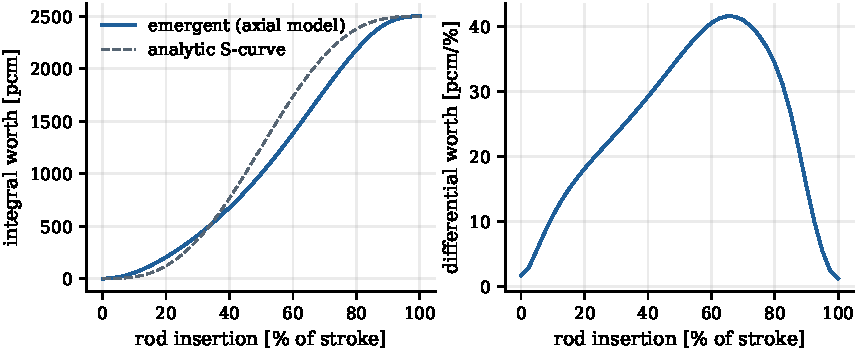
\includegraphics[width=\linewidth]{rod_worth.pdf}
  \caption{Integral (left) and differential (right) rod worth emerging from the axial
  model at full power, MOC, compared with the analytic S-curve used by the point model.}
  \label{fig:rodworth}
\end{figure}

\begin{figure}[!htbp]
  \centering
  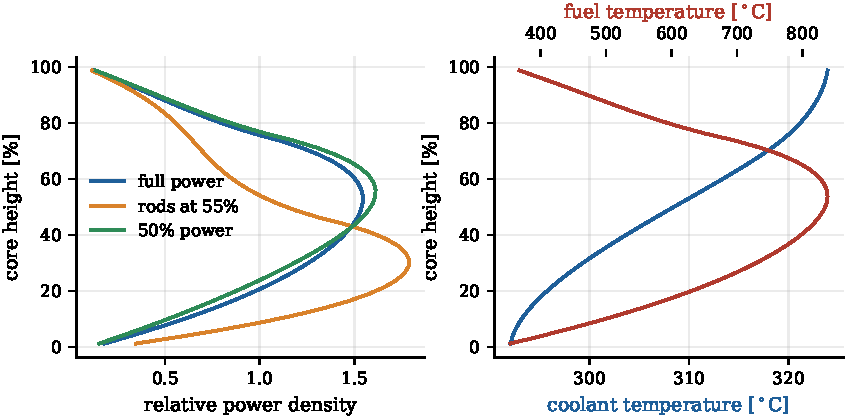
\includegraphics[width=\linewidth]{shapes.pdf}
  \caption{Left: axial power shape at full power, with the bank at 55\% insertion, and
  at 50\% power. Right: coolant and fuel temperature profiles at full power.}
  \label{fig:shapes}
\end{figure}

\begin{figure}[!htbp]
  \centering
  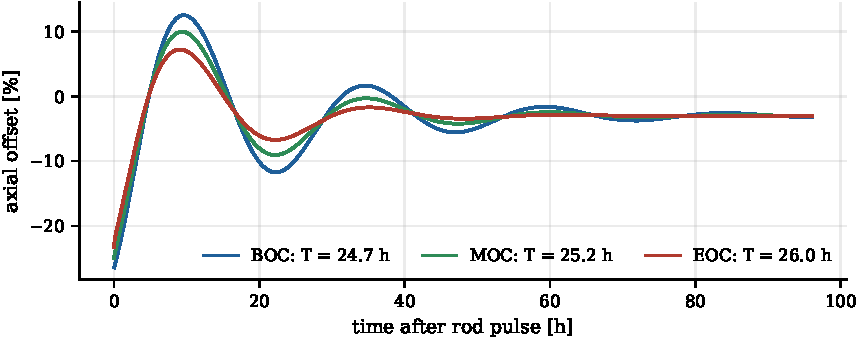
\includegraphics[width=\linewidth]{xenon_oscillation.pdf}
  \caption{Axial xenon oscillations after a rod pulse, with total power held constant by
  boron, for the three fuel-cycle states.}
  \label{fig:oscillation}
\end{figure}

\section{Steam generators and turbine}\label{sec:secondary}

In the point and axial tasks the grid demand is handed to the reactor as a power
set-point. A real PWR works differently: the grid sets the turbine, the turbine draws
steam from the steam generators, and the reactor follows the cooler or warmer water
returning to the core through its negative temperature coefficients. The optional
secondary side reproduces this chain.

\subsection{Loop equations}

Four states are added: the hot leg $T_h$, the steam-generator primary side $T_p$, the
cold leg $T_{cl}$ and the secondary saturation temperature $T_s$. The core inlet becomes
$T_{cl}$, and the core outlet is $2T_c - T_{cl}$:
\begin{align}
  \tau_h \frac{\dd T_h}{\dd t} &= 2T_c - T_{cl} - T_h,
  \qquad \tau_{cl} \frac{\dd T_{cl}}{\dd t} = T_p - T_{cl}, \\
  C_p \frac{\dd T_p}{\dd t} &= \dot m c_p\,(T_h - T_p) - UA\,(T_p - T_s), \\
  C_s \frac{\dd T_s}{\dd t} &= UA\,(T_p - T_s) - P_0\,\min\!\left(L,\; v_{max}\frac{p_{sat}(T_s)}{p_{sat}(T_{s,0})}\right).
\end{align}
The turbine governor opens its valves to draw the demanded load $L$, but at most to
$v_{max} = 1.05$ times the full-load opening, and flow through the open valves is
proportional to steam pressure. When steam pressure sags, the turbine therefore cannot
deliver its load. The saturation pressure $p_{sat}$ follows the IAPWS-IF97 region-4
equation~\cite{wagner2000}.

\subsection{Temperature program and sliding pressure}

At equilibrium the average coolant temperature follows the linear program
$T_{ref}(P) = T_{in,0} + 16\,\mathrm{K}\times P$. That is the same core temperature as
the fixed-inlet model, so the point and axial tasks are unchanged by construction. The
cold leg then stays at 292\,$^\circ$C at every load, and the conductance
$UA = P_0/(T_{cl} - T_{s,0})$ places the full-load saturation temperature at
285\,$^\circ$C. Steam pressure therefore slides from 7.66\,MPa at no load to
6.91\,MPa at full load, the familiar values of a four-loop plant. They are outputs of
the equations, not inputs.

\subsection{Self-regulation}

With rods and boron frozen, a load increase cools the steam generator, the cold leg
and the core, and the negative coefficients raise reactor power until it matches the
turbine. The new equilibrium satisfies
$\alpha_f \Delta T_f + \alpha_m \Delta T_c = 0$ with
$\Delta T_f = \Delta T_c + (T_{f,0} - T_{c,0})\,\Delta P$, so
\begin{equation}
  \Delta T_c = -\frac{\alpha_f\,(T_{f,0} - T_{c,0})}{\alpha_f + \alpha_m}\,\Delta P .
  \label{eq:selfreg}
\end{equation}
The simulator reproduces \cref{eq:selfreg} to $10^{-4}$\,K after an 80\% to 85\% load
step. For a larger step, from 90\% to 100\%, the coolant cools so much that steam
pressure falls to 6.45\,MPa, the turbine valves open fully, and the plant settles at
98.8\% of the demanded load. This is why PWRs control the average coolant
temperature rather than leaving the reactor to self-regulate.

\section{Numerical methods and verification}\label{sec:verification}

\subsection{Time integration}

The plant equations are stiff: prompt-neutron time constants are of order
milliseconds, while xenon evolves over tens of hours. The C++ core integrates them with
the two-stage, L-stable, second-order singly diagonally implicit Runge--Kutta method
of Alexander~\cite{alexander1977}:
\begin{equation}
  \begin{array}{c|cc}
    \gamma & \gamma & 0 \\
    1 & 1-\gamma & \gamma \\ \hline
      & 1-\gamma & \gamma
  \end{array}
  \qquad \gamma = 1 - \tfrac{\sqrt2}{2},
  \qquad R(z) = \frac{1 + (1 - 2\gamma)z}{(1 - \gamma z)^2}.
\end{equation}
Each stage is solved by full Newton iteration with the analytic Jacobian. The inner
step is 0.25\,s, and a step whose Newton iteration fails is halved recursively. Rod and
boron positions are integrated exactly inside each step, including the instant they
reach their limits. Local poisons in the axial core use exact exponentials for I and
Pm and the trapezoidal rule for Xe and Sm. One simulated day at a one-minute control
interval takes about one second on a laptop with the point core and about ten seconds
with the axial core.

\subsection{Independent reference}

A second implementation in Python solves the same equations with SciPy's adaptive
Radau IIA method~\cite{hairer1996,virtanen2020} at a relative tolerance of $10^{-8}$.
It uses LAPACK's tridiagonal eigensolver and exact matrix exponentials for the axial
poisons. It shares no numerical method with the C++ core, so agreement between the two
is a meaningful check.

\subsection{Verification results}

\Cref{tab:verification} lists the verification tests. All of them run in the
continuous-integration suite.

\begin{table}[!htbp]
  \centering
  \caption{Verification tests and their references.}
  \label{tab:verification}
  \small
  \begin{tabular}{@{}lll@{}}
    \toprule
    Test & Reference & Result \\
    \midrule
    Equilibrium held for 1\,h at 50\% and 100\% & exact steady state & $<10^{-9}$ \\
    Analytic Jacobian & central differences & $<10^{-5}$ rel. \\
    C++ SDIRK2 vs.\ Radau, 30\,min random actuation & independent solver & $<10^{-4}$ \\
    Prompt jump after a 0.2\$ step & $\beta/(\beta-\rho)$ & $<1\%$ \\
    Stable period, 10--400\pcm{} steps & inhour equation & $\le 0.10\%$ \\
    Xe-135 after shutdown & Bateman solution & $\le0.01\%$ \\
    Uniform local reactivity & exact global reactivity & $<10^{-12}$ \\
    Fundamental axial mode & diffusion cosine & $<2\times10^{-3}$ \\
    Eigenvalue convergence & Robin-condition solution & order 1.999 \\
    Sturm bisection vs.\ LAPACK & independent solver & $<10^{-13}$ \\
    Axial C++ vs.\ Python, 1\,h transient & independent solver & $<10^{-5}$ \\
    Coolant energy balance & $T_{out} = T_{in} + nP_0/\dot m c_p$ & $<10^{-9}$ \\
    Coupling equilibrium, $\Delta t_c$ = 60, 5, 1\,s & steady state & $<10^{-7}$ \\
    Coupling convergence in $\Delta t_c$ & finer interval & first order \\
    Rod worth table, C++ vs.\ Python & independent solver & $<10^{-12}$ \\
    Emergent total rod worth & design worth $W$ & 2501\pcm \\
    IF97 saturation pressure & standard's verification table & $<10^{-8}$ \\
    Plant steady state on the $T_{avg}$ program & exact & $<10^{-8}$ \\
    Core, steam generator and turbine energy balance & exact & $<10^{-9}$ \\
    Self-regulation after a load step & \cref{eq:selfreg} & $10^{-4}$\,K \\
    Plant C++ vs.\ Radau, 30\,min random load & independent solver & $<10^{-4}$ \\
    \bottomrule
  \end{tabular}
\end{table}

\Cref{fig:verification} shows the two kinetics tests. Stable periods from 10\pcm{} to
400\pcm{} steps agree with the largest root of the inhour
equation~\cite{hetrick1971,duderstadt1976},
\begin{equation}
  \rho = \omega\Lambda + \sum_{i=1}^{6} \frac{\beta_i\,\omega}{\omega + \lambda_i},
\end{equation}
to within 0.10\%. After a shutdown from full power, the xenon inventory follows
the closed-form solution
$X(t) = e^{-\lambda_X t} + \tfrac{\kappa\gamma_I/\gamma}{\lambda_X - \lambda_I}\left(e^{-\lambda_I t} - e^{-\lambda_X t}\right)$
to within 0.01\%, peaking at 2.66 times its equilibrium value
after 9.5\,h. \Cref{fig:convergence} confirms second-order convergence of
the axial eigenvalue to the solution of the continuous Robin problem,
$B\tan(BH/2) = 1/\delta$, $\lambda = 1 + M^2B^2$.

\begin{figure}[!htbp]
  \centering
  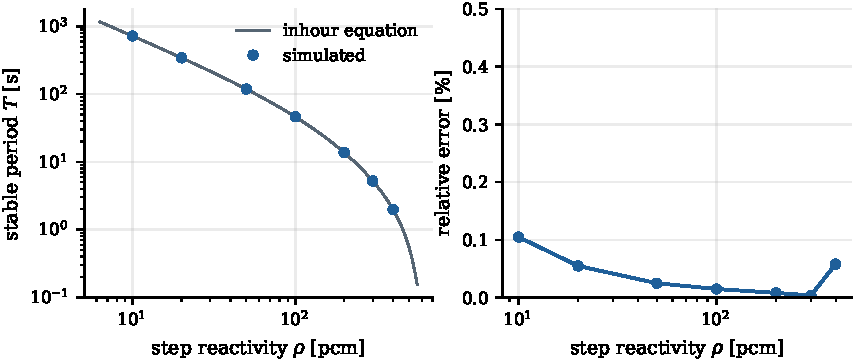
\includegraphics[width=\linewidth]{inhour.pdf}
  \caption{Stable reactor period after a reactivity step: simulation against the inhour
  equation (left) and relative error (right).}
  \label{fig:verification}
\end{figure}

\begin{figure}[!htbp]
  \centering
  \begin{subfigure}[t]{0.49\linewidth}
    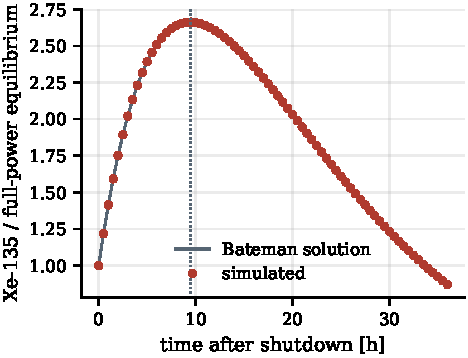
\includegraphics[width=\linewidth]{xenon_shutdown.pdf}
    \caption{Xe-135 after shutdown.}
  \end{subfigure}\hfill
  \begin{subfigure}[t]{0.49\linewidth}
    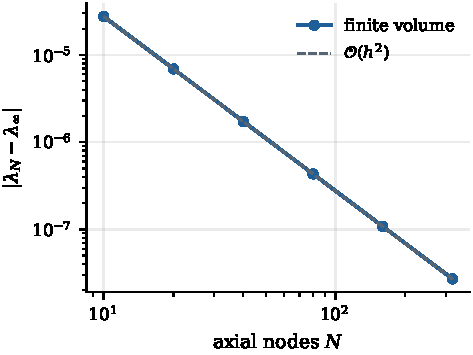
\includegraphics[width=\linewidth]{convergence.pdf}
    \caption{Eigenvalue convergence.}
  \end{subfigure}
  \caption{Verification of the poison dynamics and of the axial discretization.}
  \label{fig:convergence}
\end{figure}

\section{Benchmark task}\label{sec:task}

\subsection{Constrained Markov decision process}

Each step advances the plant by 60\,s; an episode is one day (1440 steps). The action
$\bm a\in[-1,1]^2$ sets the rod speed and the boron rate, with positive values adding
reactivity. The observation contains the measured power, the demand at the end of the
step and 15, 30 and 60 minutes ahead (a dispatch schedule), rod position, boron,
temperature deviations, xenon, iodine, reactivity in dollars, the last power rate and
episode progress. The axial task adds the axial offset, the distance from the
$\Delta I$ target band, the xenon axial offset and the peaking factor. Xenon, iodine and
reactivity are not measured directly in a plant, but core-monitoring systems estimate
them online.

The task is a CMDP~\cite{altman1999}:
\begin{equation}
  \max_\pi\; \mathbb{E}_\pi\!\left[\sum_t \gamma^t r_t\right]
  \quad\text{s.t.}\quad
  \mathbb{E}_\pi\!\left[\sum_t \gamma^t c_t\right] \le d,
\end{equation}
with tracking reward and binary safety cost
\begin{equation}
  r_t = -\min\!\left\{\left(\frac{P_t - P^{dem}_t}{0.05}\right)^{\!2}, 1\right\} - 0.005\,\lVert\bm a_t\rVert_1,
  \qquad
  c_t = \mathbf{1}\!\left[\text{any limit in \cref{tab:limits} violated in step } t\right].
\end{equation}
A peak power above 109\% trips the reactor and ends the episode. To remove any
incentive to end an episode early, the trip reward equals the discounted value of
losing every remaining step:
\begin{equation}
  r_{trip} = -\sum_{j=0}^{k-1}\gamma^j = -\frac{1-\gamma^{k}}{1-\gamma},
\end{equation}
where $k$ is the number of remaining steps.

\begin{table}[!htbp]
  \centering
  \caption{Operating limits that define the safety cost.}
  \label{tab:limits}
  \small
  \begin{tabular}{@{}lll@{}}
    \toprule
    Limit & Threshold & Purpose \\
    \midrule
    Overpower & peak power in step $>105\%$ & thermal margin \\
    Ramp rate & $|\Delta P| > 5\%$ of rated per minute & manoeuvrability limit~\cite{eur} \\
    Fuel temperature & average fuel $>690\,^\circ$C & fuel thermal margin \\
    Axial offset (axial task) & $|\Delta I - \Delta I_{target}| > 5\%$ & power-distribution margin \\
    Steam pressure (plant task) & outside 5.5--8.0\,MPa & turbine supply, relief valves \\
    Trip (terminal) & peak power $>109\%$ & reactor protection \\
    \bottomrule
  \end{tabular}
\end{table}

\subsection{Plant task}

With the secondary side enabled, the demand drives the turbine and the tracking error
is measured on turbine output. The observation gains the turbine output, the deviation
$T_{avg} - T_{ref}$, the steam pressure and the cold-leg temperature, and the reward
adds $-0.2\min\{(\Delta T_{avg}/5\,\mathrm{K})^2, 1\}$. The plant and axial options
combine.

\subsection{Scenarios and protocol}

Four demand scenarios are evaluated:
\begin{itemize}
  \item \emph{EUR daily}: 12\,h at 100\%, a 3\,h ramp to 50\%, 6\,h at 50\% and a
  3\,h ramp back~\cite{eur}.
  \item \emph{Fast ramp}: 100$\to$50$\to$100\% at 5\%/min, followed by the long xenon
  transient.
  \item \emph{Duck curve}: the net load left after solar and wind generation.
  \item \emph{Frequency response}: secondary frequency-control set-point steps near
  full power.
\end{itemize}
A result is the mean over 4 scenarios $\times$ 3 cycle states $\times$ 3 seeds
(36 episodes). The reported metrics are tracking RMSE and maximum error, time within
$\pm1\%$, energy deficit, rod travel, boron used, safety-cost steps, trips and, for the
axial task, $\Delta I$ deviation and peaking.

\section{Baseline controllers}\label{sec:baselines}

\paragraph{Classical controller (PID).} It mirrors the usual PWR split between fast
rods and slow boron. With power error $e = P^{dem}_{t+1} - P_t$, its integral $I$, and
the preview slope $s = (P^{dem}_{t+15} - P^{dem}_{t+1})/14$, the controller requests the
reactivity change
$\Delta\rho = \bar\alpha_P\,(k_p e + k_i I + s)$. Here $\bar\alpha_P$ is a nominal
power coefficient. This request is converted into a rod displacement through the local
differential worth, $\Delta z = \Delta\rho / W(1 - \cos 2\pi z)$, with a deadband to
limit rod wear. A slow boron loop returns the rods to a reference band:
$u_B = -k_B\,(z - z_{ref} \mp z_{band})$ outside the band. The controller ignores the
axial power distribution.

\paragraph{Temperature controller.} For the plant task, a controller in the style of
PWR rod control acts on the temperature error $e_T = T_{ref}(L) - T_{avg}$ and on the
power mismatch $L - P$ between turbine and reactor. It requests
$\Delta\rho = k_T\,\bar\alpha_T\,e_T + k_P\,\bar\alpha_P\,(L - P)$, with a 0.8\,K deadband
on $e_T$, converts the request into a rod displacement exactly as the PID does, and uses
the same boron loop to keep the bank in its band.

\paragraph{Soft Actor-Critic (SAC).} A model-free agent with a tanh-squashed Gaussian
policy, twin critics and automatic entropy tuning~\cite{haarnoja2018}. It is trained
on randomized demand profiles and cycle states with observation noise. The released
checkpoint was trained for 179 simulated plant-days on the point task, before the
core-average flux was raised from $3\times10^{13}$ to its present value. It therefore
operates on slightly different xenon dynamics than it learned, and it is reported
here as a reference point rather than a tuned result.

\paragraph{Runtime-assurance shield.} Following the Simplex
architecture~\cite{sha2001}, the shield (\cref{alg:shield}) simulates each proposed
action one step ahead on a copy of the plant. If the prediction violates a limit, it
substitutes the least-modified safe alternative: first scaled-down versions of the
proposal, then the classical controller's action, then holding still. Interventions
are counted and reported.

\begin{algorithm}[!htbp]
  \caption{One-step runtime-assurance shield}
  \label{alg:shield}
  \begin{algorithmic}[1]
    \Require plant state $s$, proposed action $\bm a$, fallback action $\bm a_f$
    \State $v \gets \textsc{Severity}(\textsc{Predict}(s, \bm a))$
    \If{$v = 0$} \Return $\bm a$ \EndIf
    \For{$\bm a' \in (0.5\bm a,\; 0.25\bm a,\; 0.1\bm a,\; \bm a_f,\; \bm 0)$}
      \State $v' \gets \textsc{Severity}(\textsc{Predict}(s, \bm a'))$
      \If{$v' < v$} $(\bm a, v) \gets (\bm a', v')$ \EndIf
      \If{$v' = 0$} \textbf{break} \EndIf
    \EndFor
    \State \Return $\bm a$ \Comment{Severity: $10\times$trip $+$ number of violated limits}
  \end{algorithmic}
\end{algorithm}

\section{Results}\label{sec:results}

\Cref{tab:results-point} reports the point task. The classical controller tracks power
to within 0.22\% RMS on its best scenario, with no trips. On the fast-ramp
scenario its error reaches 22.7\% after the return to full power
(\cref{fig:episode}). By then xenon is high, the rods have run out of withdrawal travel,
and dilution at 3\,ppm/min is too slow to catch up. A controller that used the dispatch
preview and the iodine inventory to dilute ahead of the ramp could close this gap.
Anticipation of this kind is exactly what learned and model-predictive controllers
should be able to provide.

SAC tracks power far worse than the classical controller and trips the reactor in
5 of 36 benchmark days. With the shield it trips
0 times, with 0 cost steps in total, and its error drops
on every scenario. The result separates two properties that are often conflated:
runtime assurance can make a learned policy \emph{safe to evaluate}, but it does not
make the policy \emph{good}.

\Cref{tab:results-axial} reports the axial task. The classical controller still tracks
total power to within 0.61\% RMS. Because it ignores the power shape, however,
it leaves the $\Delta I$ band in 39\% of all minutes, and the axial
peaking factor reaches 2.00. \Cref{fig:axial-episode} shows the mechanism.
Rod insertion during the power reduction pushes power toward the bottom, and xenon then
accumulates in the lower half. Once the rods are withdrawn, the power swings to the top
of the core. Following load while holding the power distribution is therefore the
central open problem the benchmark poses.


\begin{table}[!htbp]
  \centering
  \caption{Point task. Means over three cycle states and three seeds per scenario.}
  \label{tab:results-point}
  \small
  \begin{tabular}{@{}llrrrrr@{}}
    \toprule
    Controller & Scenario & RMSE [\%] & Max err.\ [\%] & Within 1\% [\%] & Cost steps & Trips \\
    \midrule
    PID & EUR daily & 0.22 & 0.6 & 100.0 & 0.0 & 0/9 \\
 & Fast ramp & 1.34 & 17.3 & 94.8 & 1.7 & 0/9 \\
 & Duck curve & 0.23 & 1.0 & 99.9 & 0.0 & 0/9 \\
 & Frequency & 0.29 & 1.0 & 99.2 & 0.0 & 0/9 \\
\midrule
PID + shield & EUR daily & 0.22 & 0.6 & 100.0 & 0.0 & 0/9 \\
 & Fast ramp & 1.32 & 16.0 & 94.8 & 0.0 & 0/9 \\
 & Duck curve & 0.23 & 1.0 & 99.9 & 0.0 & 0/9 \\
 & Frequency & 0.29 & 1.0 & 99.2 & 0.0 & 0/9 \\
\midrule
Hold & EUR daily & 28.87 & 50.0 & 50.5 & 0.0 & 0/9 \\
 & Fast ramp & 20.70 & 50.0 & 82.0 & 0.0 & 0/9 \\
 & Duck curve & 21.28 & 47.7 & 28.8 & 0.0 & 0/9 \\
 & Frequency & 3.43 & 6.2 & 17.9 & 0.0 & 0/9 \\
\midrule
SAC & EUR daily & 2.98 & 29.9 & 33.7 & 6.3 & 0/9 \\
 & Fast ramp & 31.41 & 61.2 & 21.9 & 6.3 & 0/9 \\
 & Duck curve & 34.79 & 50.5 & 24.7 & 4.4 & 3/9 \\
 & Frequency & 22.64 & 30.8 & 26.3 & 2.6 & 2/9 \\
\midrule
SAC + shield & EUR daily & 2.79 & 7.4 & 33.8 & 0.0 & 0/9 \\
 & Fast ramp & 31.27 & 50.7 & 22.0 & 0.0 & 0/9 \\
 & Duck curve & 2.12 & 6.1 & 32.7 & 0.0 & 0/9 \\
 & Frequency & 2.26 & 10.4 & 34.4 & 0.0 & 0/9 \\
\bottomrule
  \end{tabular}
\end{table}

\begin{table}[!htbp]
  \centering
  \caption{Axial task. $\Delta I$ violations are minutes outside the band, per day.}
  \label{tab:results-axial}
  \small
  \begin{tabular}{@{}llrrrrr@{}}
    \toprule
    Controller & Scenario & RMSE [\%] & $\Delta I$ RMS dev.\ [\%] & $\Delta I$ viol.\ [min] & Max $F_z$ & Trips \\
    \midrule
    PID & EUR daily & 0.21 & 11.57 & 579 & 1.99 & 0/9 \\
 & Fast ramp & 1.70 & 12.57 & 955 & 2.00 & 0/9 \\
 & Duck curve & 0.22 & 10.10 & 698 & 1.86 & 0/9 \\
 & Frequency & 0.29 & 2.34 & 42 & 1.61 & 0/9 \\
\midrule
PID + shield & EUR daily & 0.22 & 11.57 & 577 & 1.99 & 0/9 \\
 & Fast ramp & 2.86 & 12.55 & 936 & 1.98 & 0/9 \\
 & Duck curve & 0.68 & 9.35 & 650 & 1.85 & 0/9 \\
 & Frequency & 0.30 & 2.34 & 36 & 1.61 & 0/9 \\
\midrule
Hold & EUR daily & 28.87 & 0.00 & 0 & 1.56 & 0/9 \\
 & Fast ramp & 20.70 & 0.00 & 0 & 1.56 & 0/9 \\
 & Duck curve & 21.28 & 0.00 & 0 & 1.56 & 0/9 \\
 & Frequency & 3.43 & 0.72 & 0 & 1.57 & 0/9 \\
\bottomrule
  \end{tabular}
\end{table}

\begin{figure}[!htbp]
  \centering
  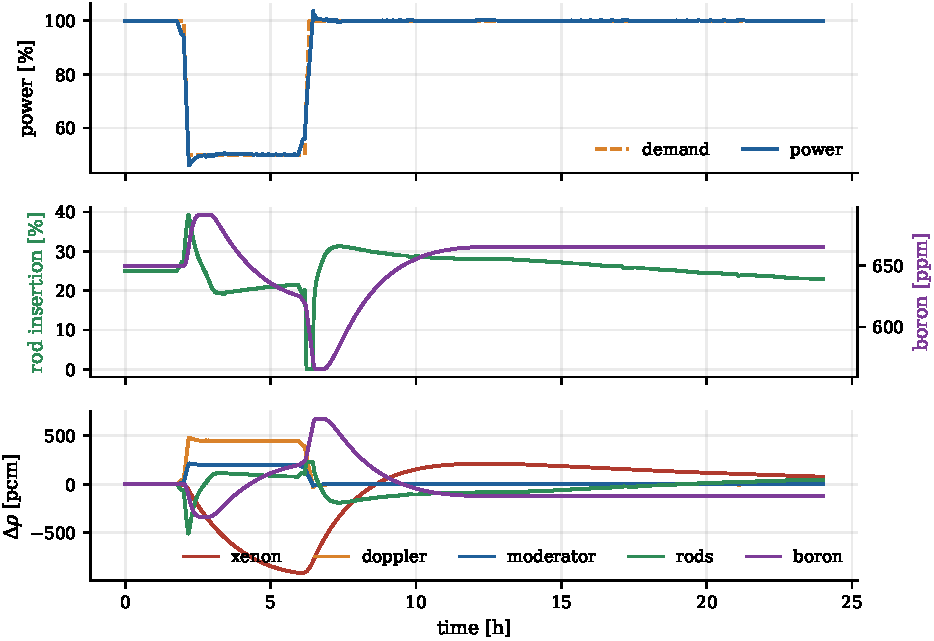
\includegraphics[width=\linewidth]{episode_fast_ramp.pdf}
  \caption{Classical controller on the fast-ramp scenario, MOC. Top: demand and power.
  Middle: rod insertion and boron. Bottom: reactivity contributions relative to the
  initial state.}
  \label{fig:episode}
\end{figure}

\begin{figure}[!htbp]
  \centering
  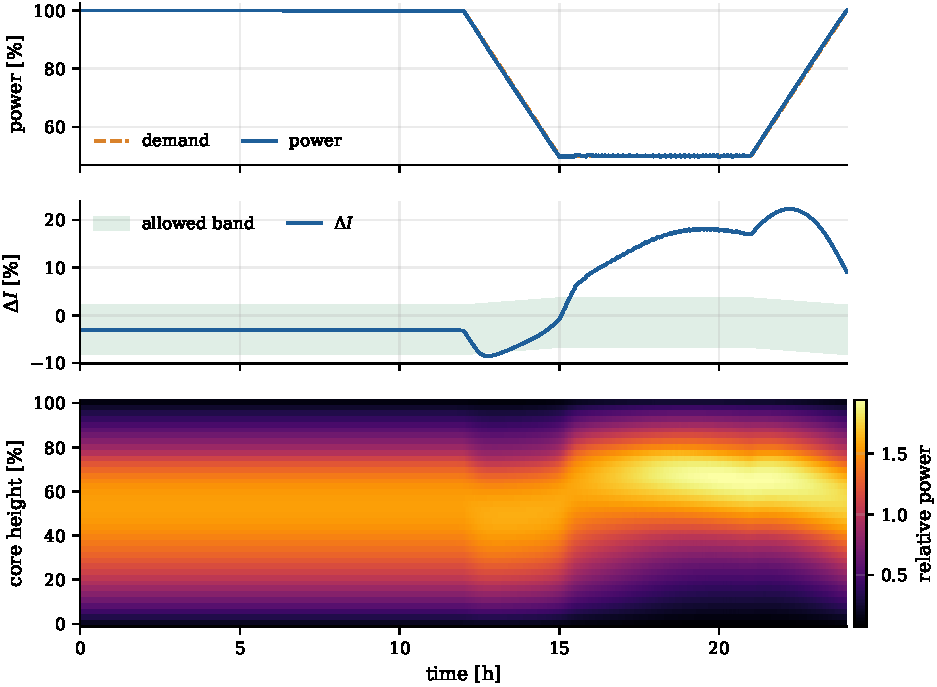
\includegraphics[width=\linewidth]{episode_axial.pdf}
  \caption{Classical controller on the EUR daily cycle with the axial core, MOC. The
  power shape (bottom) moves down during the rod insertion and then to the top as
  xenon redistributes, carrying $\Delta I$ (middle) out of its band.}
  \label{fig:axial-episode}
\end{figure}

\paragraph{Plant task.} \Cref{tab:results-plant} reports the plant task. With the
turbine in the loop, every controller delivers the demanded electrical power on most
scenarios, because the reactor self-regulates. Even holding the rods still tracks the
grid to within 0.01\% on three scenarios. The difference lies in what happens to the
plant meanwhile (\cref{fig:plant}). A controller that drives reactor power to the
demand, the natural strategy on the point task, leaves the temperature unanchored:
$T_{avg}$ drifts up to 50\,K off its program, and steam pressure swings between 3.3 and
9.6\,MPa. A temperature controller holds $T_{avg}$ within 1\,K and steam pressure inside
its limits on three scenarios. The remaining difficulty is again the fast return to
power: steam pressure sags to 6.2\,MPa, the turbine valves open fully and $T_{avg}$
falls by up to 8\,K before the rods catch up.

\begin{table}[!htbp]
  \centering
  \caption{Plant task. $T_{avg}$ is the deviation from its program; steam pressure is
  the range over the nine days of each scenario.}
  \label{tab:results-plant}
  \footnotesize
  \begin{tabular}{@{}llrrrrr@{}}
    \toprule
    Controller & Scenario & Output RMSE [\%] & $T_{avg}$ RMS [K] & $T_{avg}$ max [K] & Steam [MPa] & Cost \\
    \midrule
    Temperature & EUR daily & 0.00 & 0.46 & 1.0 & 6.91--7.37 & 0.0 \\
     & Fast ramp & 0.21 & 0.82 & 8.3 & 6.21--7.43 & 12.7 \\
     & Duck curve & 0.00 & 0.52 & 1.0 & 6.83--7.35 & 0.0 \\
     & Frequency & 0.00 & 0.42 & 0.8 & 6.85--7.09 & 0.0 \\
    \midrule
    Temperature & EUR daily & 0.00 & 0.46 & 1.0 & 6.91--7.37 & 0.0 \\
    + shield & Fast ramp & 0.47 & 1.14 & 15.3 & 5.66--7.98 & 1.7 \\
     & Duck curve & 0.00 & 0.52 & 1.0 & 6.83--7.35 & 0.0 \\
     & Frequency & 0.00 & 0.42 & 0.8 & 6.85--7.09 & 0.0 \\
    \midrule
    Power (PID) & EUR daily & 0.04 & 24.20 & 49.7 & 3.28--9.61 & 550.0 \\
     & Fast ramp & 3.34 & 16.78 & 46.5 & 3.46--8.34 & 587.7 \\
     & Duck curve & 0.01 & 11.45 & 27.2 & 4.79--7.99 & 272.8 \\
     & Frequency & 0.04 & 4.20 & 12.3 & 5.81--7.51 & 0.0 \\
    \midrule
    Hold & EUR daily & 0.00 & 7.36 & 30.6 & 4.53--8.14 & 153.7 \\
     & Fast ramp & 5.57 & 10.49 & 44.0 & 3.95--11.27 & 402.3 \\
     & Duck curve & 0.00 & 7.15 & 29.3 & 4.56--9.58 & 228.0 \\
     & Frequency & 0.01 & 1.50 & 6.0 & 6.38--7.64 & 0.0 \\
    \bottomrule
  \end{tabular}
\end{table}

\begin{figure}[!htbp]
  \centering
  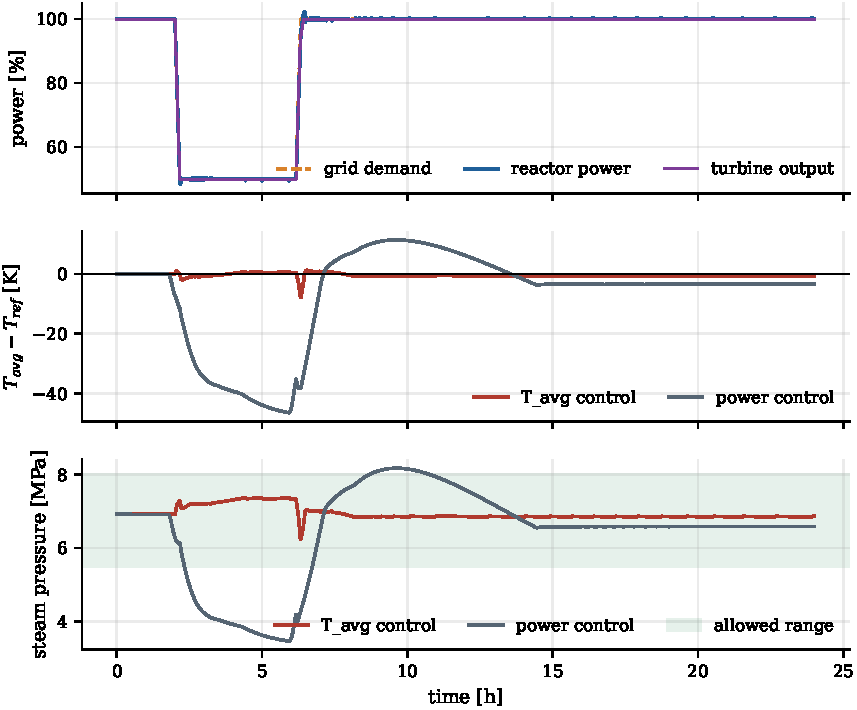
\includegraphics[width=\linewidth]{plant_fast_ramp.pdf}
  \caption{Plant task, fast ramp, MOC. Top: grid demand, reactor power and turbine
  output under temperature control. Middle and bottom: deviation of $T_{avg}$ from its
  program and steam pressure, for temperature control and for power control.}
  \label{fig:plant}
\end{figure}

\section{Limitations}\label{sec:limitations}

\Norman{} is a research benchmark. It is not a safety-analysis code, and it has not
been validated against plant data. Its main simplifications are:
\begin{itemize}
  \item a one-group, one-dimensional shape, with no radial or energy dependence;
  \item a single lumped rod bank, with burnup represented by a linear axial tilt;
  \item a quasi-static shape with first-order coupling every 5\,s, which is accurate for
  xenon- and rod-driven changes but not for sub-second spatial transients;
  \item a lumped secondary side, with one steam-generator node for four loops, no level
  dynamics and no pressurizer;
  \item boron that acts instantly in the core;
  \item representative rather than plant-specific parameters.
\end{itemize}
A model-predictive baseline and constrained reinforcement learning baselines are under
development in the same repository.

\section{Conclusion}

We have presented an open benchmark for PWR load-following control whose plant is
documented, verified against analytic results and checked by an independent
implementation. Its axial core reproduces day-long xenon oscillations and an emergent,
skewed rod worth curve. Its CMDP formulation separates safety from performance. The
baselines expose two clear gaps: anticipating xenon after fast power changes, and
controlling the axial power distribution during load following. We hope that a shared,
checkable plant will help results on learned and classical reactor controllers become
comparable, and that review by reactor engineers will improve the model further.

\paragraph{Reproducibility.} The code, per-episode results and the trained checkpoint
are available at the repository above. Every result table can be reproduced with
\texttt{norman evaluate}, and the verification tests run with \texttt{pytest}.

\renewcommand{\bibfont}{\small\raggedright}
\bibliographystyle{unsrtnat}
\bibliography{references}

\end{document}
